\documentclass[12pt]{article}

\usepackage[T2A]{fontenc}
\usepackage[utf8x]{inputenc}
\usepackage[english, russian]{babel}
\usepackage{geometry}
\geometry{a4paper, portrait, margin=0.75in}

\usepackage{authoraftertitle}
\usepackage[normalem]{ulem}
\usepackage{fixltx2e}
\usepackage{float}
\usepackage{enumitem}
\usepackage{setspace}
\usepackage{graphicx}
\usepackage[table]{xcolor}
\usepackage{transparent}
\usepackage{bm}

\usepackage{caption}
\usepackage{subcaption}

\usepackage{amsmath}
% Change * to \dot
\DeclareMathSymbol{*}{\mathbin}{symbols}{"01}

\definecolor{aquamarine}{rgb}{127,255,212}
\newcolumntype{e}{>{\columncolor{yellow}}c}

\usepackage{listings}
\usepackage{color}
\def\matlab{/mnt/c/University/CAPR/MATLAB/}
\definecolor{MLgreen}{RGB}{28,172,0} % color values Red, Green, Blue
\definecolor{MLlilas}{RGB}{170,55,241}
\lstset{language=Matlab,%
    %basicstyle=\color{red},
    basicstyle=\footnotesize\fontfamily{cmr},
    breaklines=true,%
    morekeywords={matlab2tikz},
    keywordstyle=\color{blue},%
    morekeywords=[2]{1}, keywordstyle=[2]{\color{black}},
    identifierstyle=\color{black},%
    stringstyle=\color{MLlilas},
    commentstyle=\color{MLgreen},%
    showstringspaces=false,%without this there will be a symbol in the places where there is a space
    numbers=left,%
    numberstyle={\tiny \color{black}},% size of the numbers
    numbersep=9pt, % this defines how far the numbers are from the text
    emph=[1]{for,end,break},emphstyle=[1]\color{red}, %some words to emphasise
    %emph=[2]{word1,word2}, emphstyle=[2]{style},
    frame = single,
}

\usepackage{hyperref}
\hypersetup{
    colorlinks,
    citecolor=black,
    filecolor=black,
    linkcolor=black,
    urlcolor=blue,
}

\begin{document}

\begin{titlepage}
    \begingroup
\fontsize{12pt}{14pt}\selectfont

\begin{center}

    Санкт-Петербургский политехнический университет имени Петра великого\\
    Институт компьютерных наук и кибербезопасности\\
    Высшая школа компьютерных технологий и информационных систем\\

    \vspace{\fill}

    \onehalfspacing
    \textbf{\huge Лабораторная работа \textnumero 12}\\
    \medbreak
    Дисциплина:\textbf{ Телекоммуникационные технологии}\\
    Тема: \textbf{ Изменение частоты дискретизации}\\
    \vspace{1.5cm}
\end{center}


\begin{flushright}
    \doublespacing
    Выполнил студент гр. 5130901{\textbackslash}10201 \underline{\hspace{7em}} Рубцов Е.А.\\
    \smallskip
    Принял преподаватель \uline{\hspace{7em}}Богач Н.В. \\
    \smallskip
    "\uline{\hspace{1.5em}}" \uline{\hspace{5em}} 2024 г.\\
\end{flushright}

\vspace{\fill}

\begin{center}
    Санкт-Петербург\\
    2024 г.\\
\end{center}

\singlespacing

\pagebreak

\endgroup


\end{titlepage}

\tableofcontents
\pagebreak

\section{Задание}
\begin{flushleft}
    Дата рождения: \textit{23.08.2003}\break
    Номер варианта: \textit{3} \break
    Статья: \textit{\href{https://wiki.gnuradio.org/index.php?title=Sample\_Rate\_Change}{Sample Rate Change}}
\end{flushleft}
Для выполнения данного задания использовалась программа \textit{Gnu Radio} версии 3.9.4

\section{Интерполяция}
\textit{Интерполяция} --- это процесс увеличения частоты дискретизации и, следовательно,
доступной полосы пропускания.

В данной лабораторной работе я буду увеличивать частоту дискретизации при помощи блока \textit{Interpolating FIR Filter.}.

\begin{figure}[H]
    \centering
    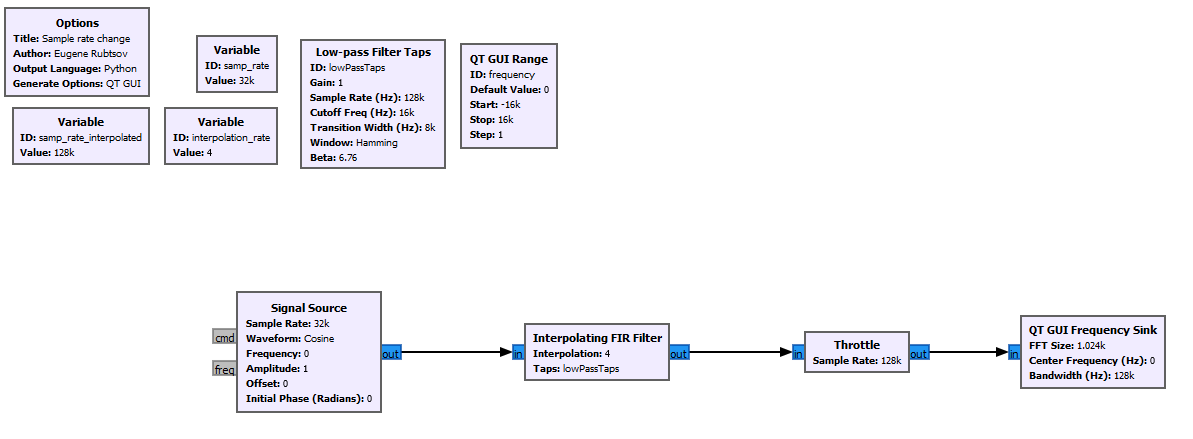
\includegraphics[width=1\textwidth]{images/inter-block.png}
    \caption{Блок-схема интерполяции}
\end{figure}

Вышепредставленная схема состоит из следующих блоков
\begin{enumerate}
    \item Два блока с переменными \textit{interpolation\_rate} и \textit{samp\_rate}
    \item \textit{Low-Pass Filter}, который пропускает сигналы только ниже определенной частоты. В данном случае используется
    чтобы уменьшить искажения результирующего сигнала
    \item \textit{QT GUI Range}, который во время исполнения кода позволяет изменять некоторую переменную в определенном диапазоне
    \item \textit{Signal Source} --- это источник сигнала, к которому применяется интерполяция
    \item \textit{Interpolating FIR Filter} -- это блок, который применяет \textit{Low-Pass Filter} к сигналу
    \item \textit{Throttle} позволяет ограничить пропуск сэмплов до определенной частоты
    \item \textit{QT GUI Frequency Sink} позволяет вывести полученный сигнал на экран
\end{enumerate}

После применения данного фильтра, был получен следующий результат:
\begin{figure}[H]
    \centering
    \begin{subfigure}[t]{0.48\textwidth}
        \centering
        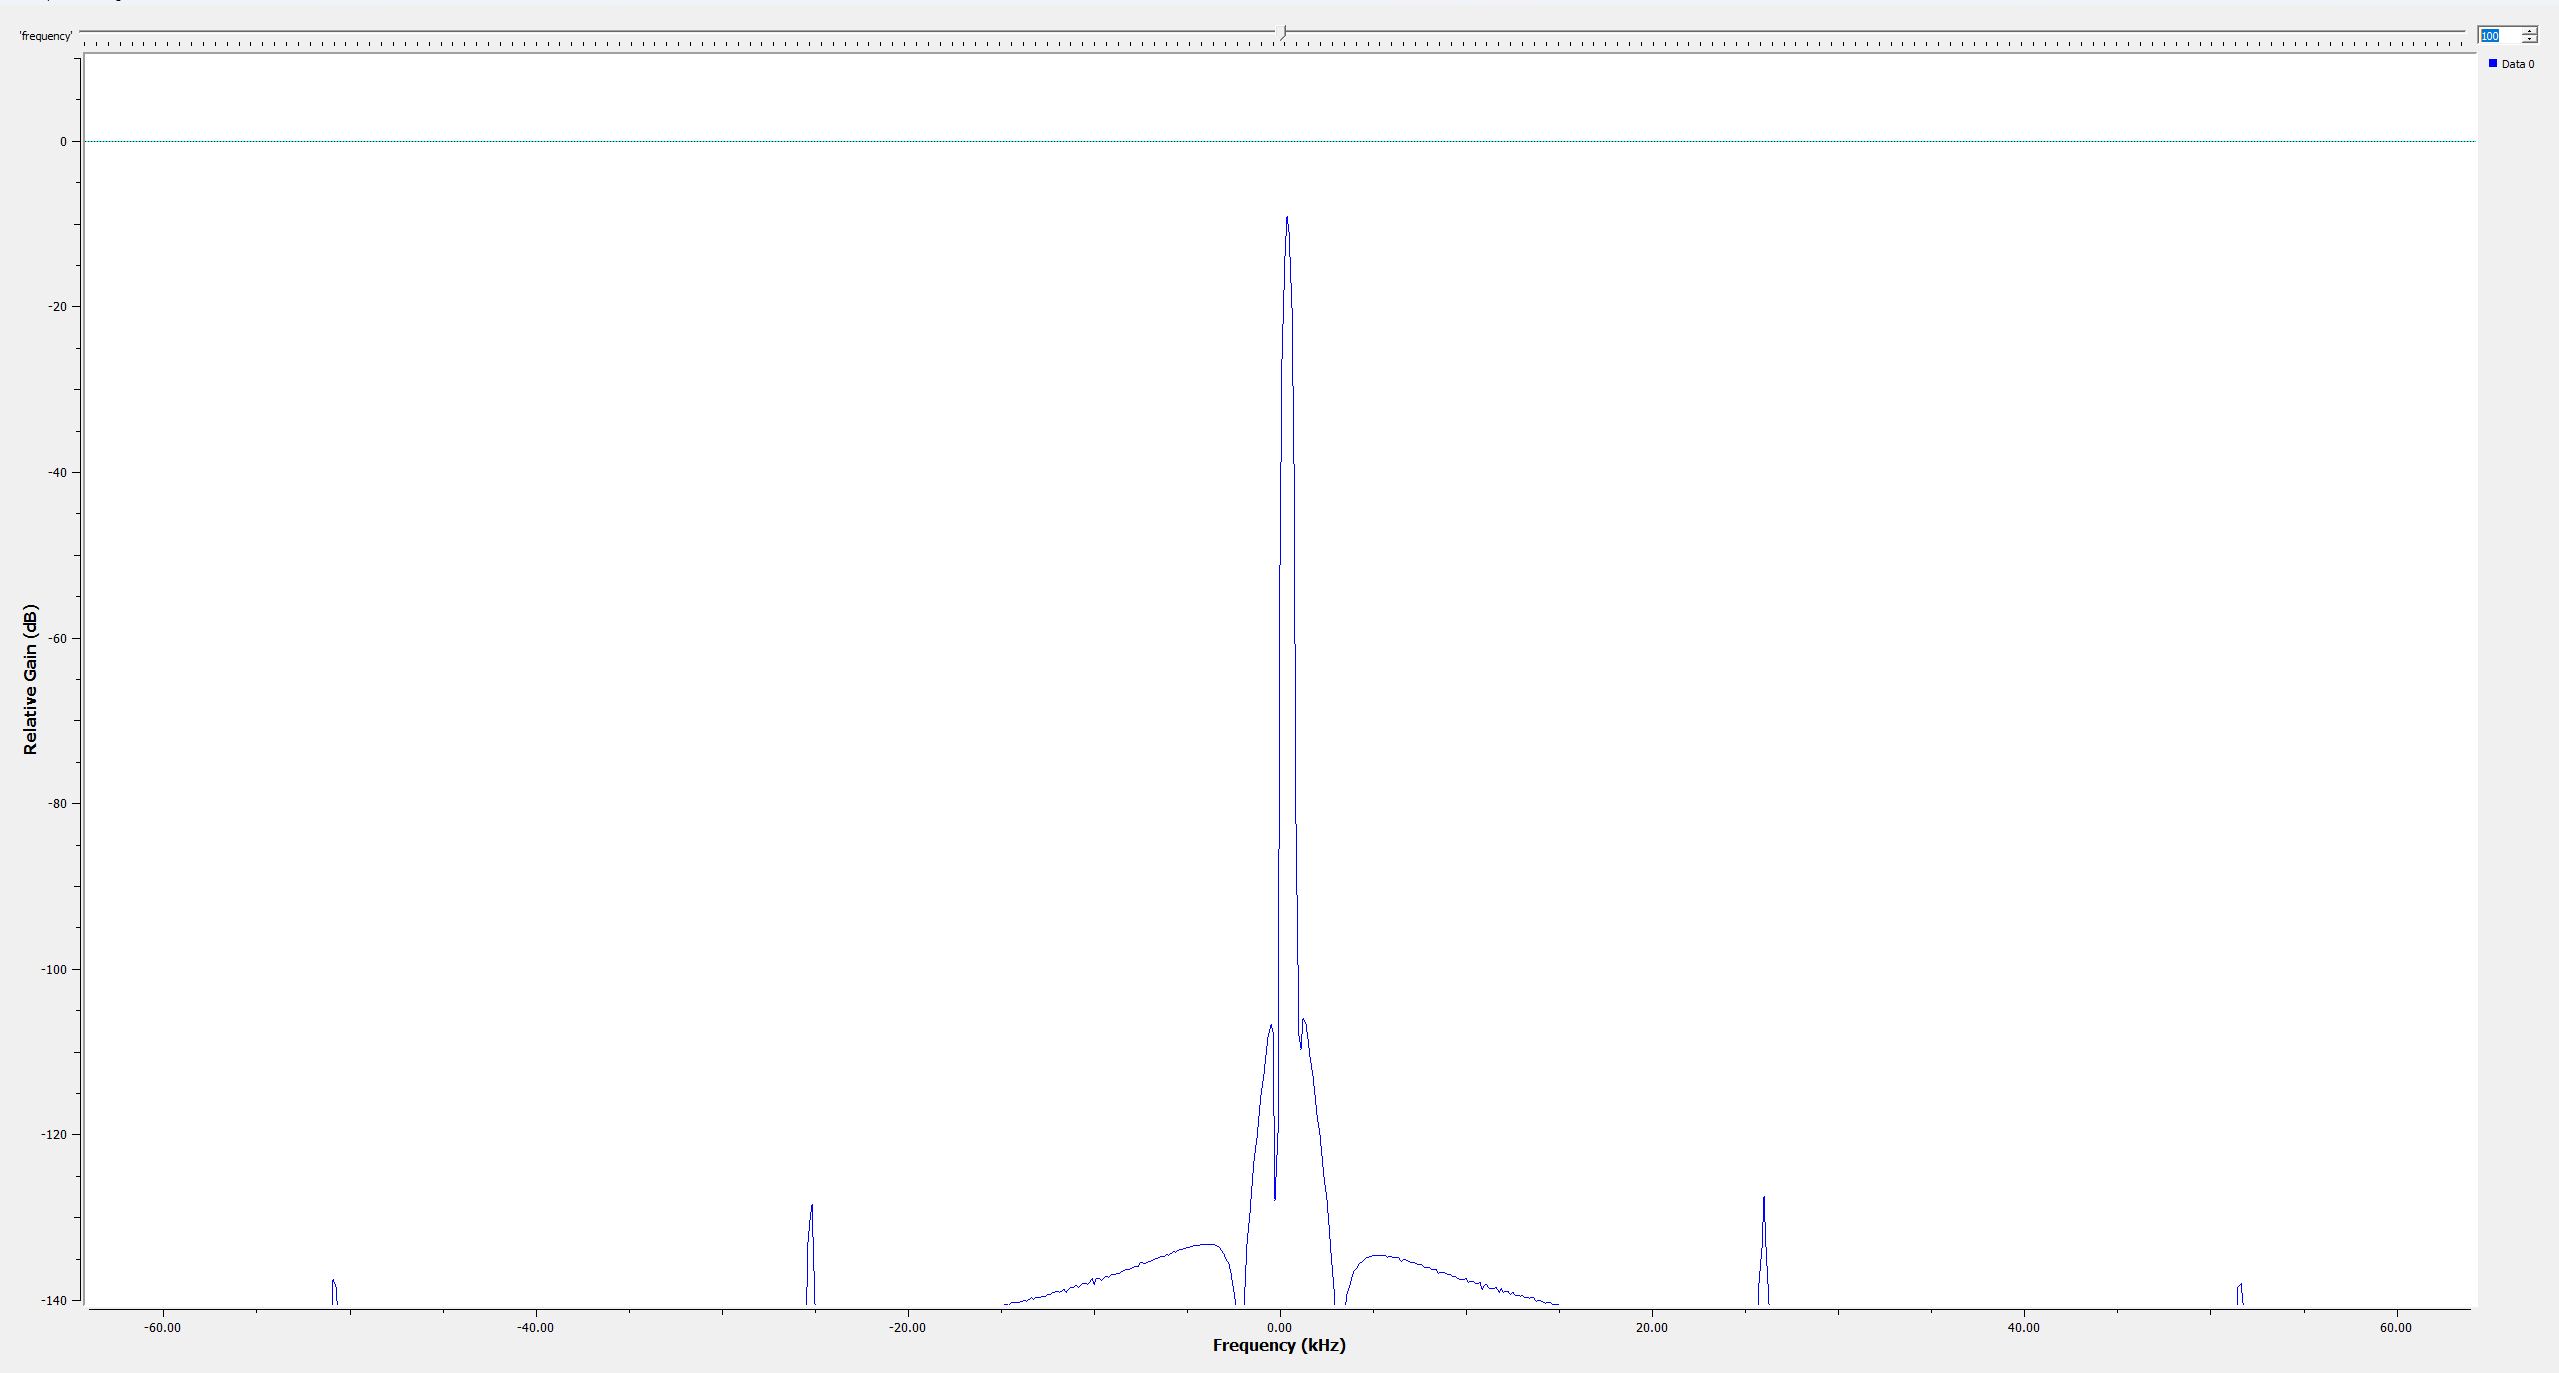
\includegraphics[width=\textwidth]{images/source-signal.png}
        \caption{Исходный сигнал}
    \end{subfigure}
    \hfill
    \begin{subfigure}[t]{0.48\textwidth}
        \centering
        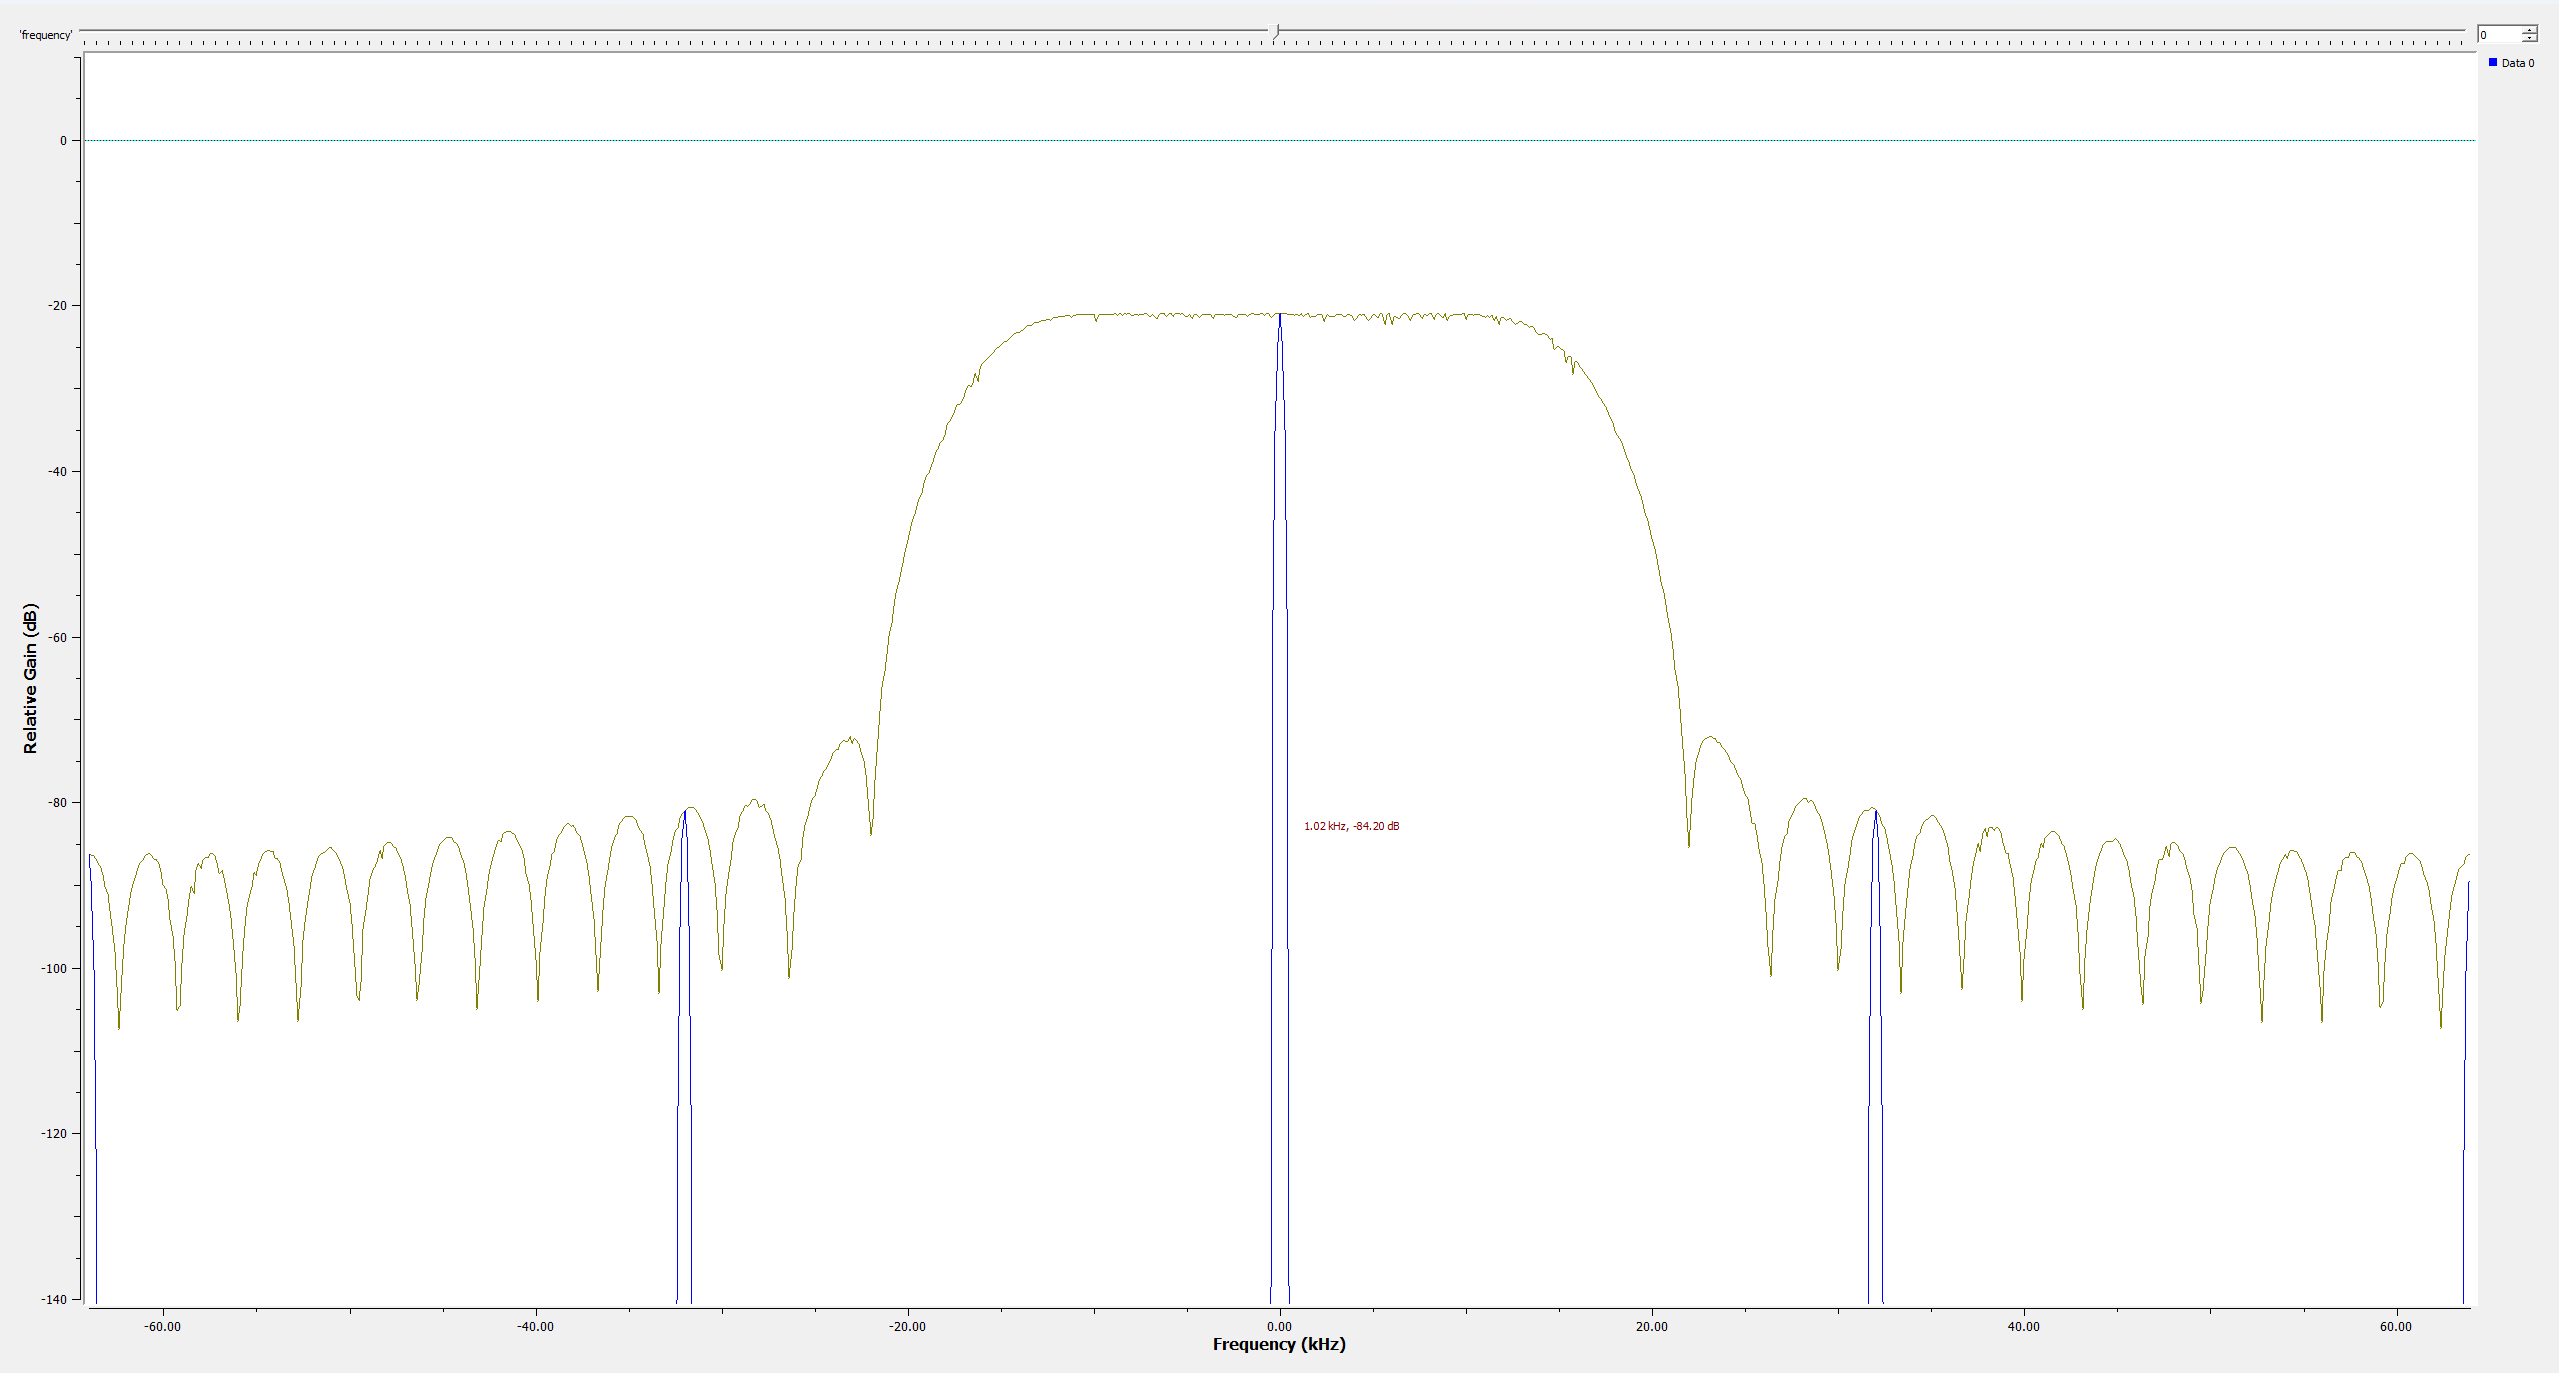
\includegraphics[width=\textwidth]{images/freq-responce.png}
        \caption{Интерполированный сигнал}
    \end{subfigure}
    \caption{Интерполяция сигнала}
\end{figure}

Как видно из изображений, после интерполяции на графике появилось 4 пика.

\section{Децимация}
\textit{Децимация} --- это процесс уменьшения частоты дискретизации путем прореживания отсчетов сигнала

Для реализации эффекта децимации средствами GNU Radio используется данная блок-схема:
\begin{figure}[H]
    \centering
    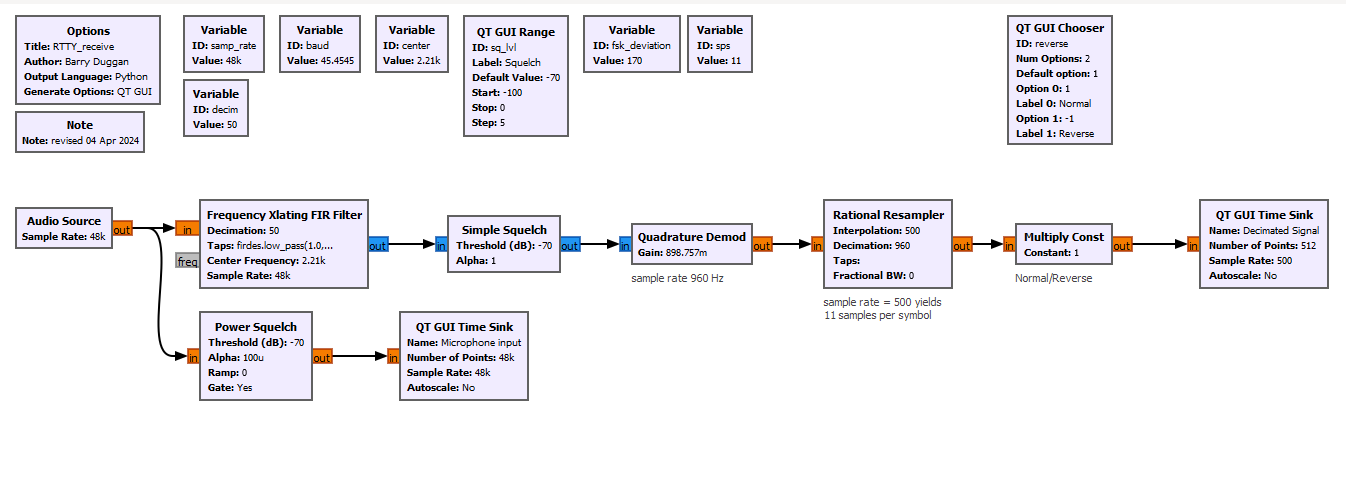
\includegraphics[width=1\textwidth]{images/decim-block.png}
    \caption{Блок-схема децимации}
\end{figure}

\textbf{\large Принцип работы схемы:}\medbreak

\begin{enumerate}
    \item Тональные сигналы частотной манипуляции (FSK) поступают с микрофона компьютера с частотой дискретизации 48 кГц.
    Эти данные подаются на \textit{Frequency Xlating FIR Filter}() с оксированием частоты, который смещает тоны выше и ниже центральной частоты.
    Он также делит частоту дискретизации на 50, получая выходную частоту дискретизации равную 960.

    \item Блок \textit{Quadrature Demod} принимает поток комплексных выборок, таких как узкий поток модулирующих сигналов, содержащий требуемый сигнал,
    и создает поток чисел с плавающей запятой, представляющих демодуляцию частоты.

    \item Время символа RTTY, по определению, составляет ровно 22 мс, что дает знакомые 45 бод (1/0,022 округления).
    Чтобы получить целое число выборок на символ, была выбрана частота выборки 500, что дает 11 выборок на символ времени.
    (500 выборок/сек * 0,022 секунды = 11 отсчетов).

    \item Выход блока \textit{Quadrature Demod} имеет частоту дискретизации 960; Желаемая частота дискретизации — 500. \textit{Rational Resampler} интерполирует (умножает)
    частоту дискретизации на 500 и прореживает (делит) ее на 960, чтобы получить выходную частоту дискретизации 500.

    \item Двоичный срез выдает выходные данные +1 для входных данных, превышающих ноль, и 0 для входных данных, меньших нуля.
\end{enumerate}

После применения данного фильтра к сигналу микрофона, получаем следующий сигнал

\begin{figure}[H]
    \centering
    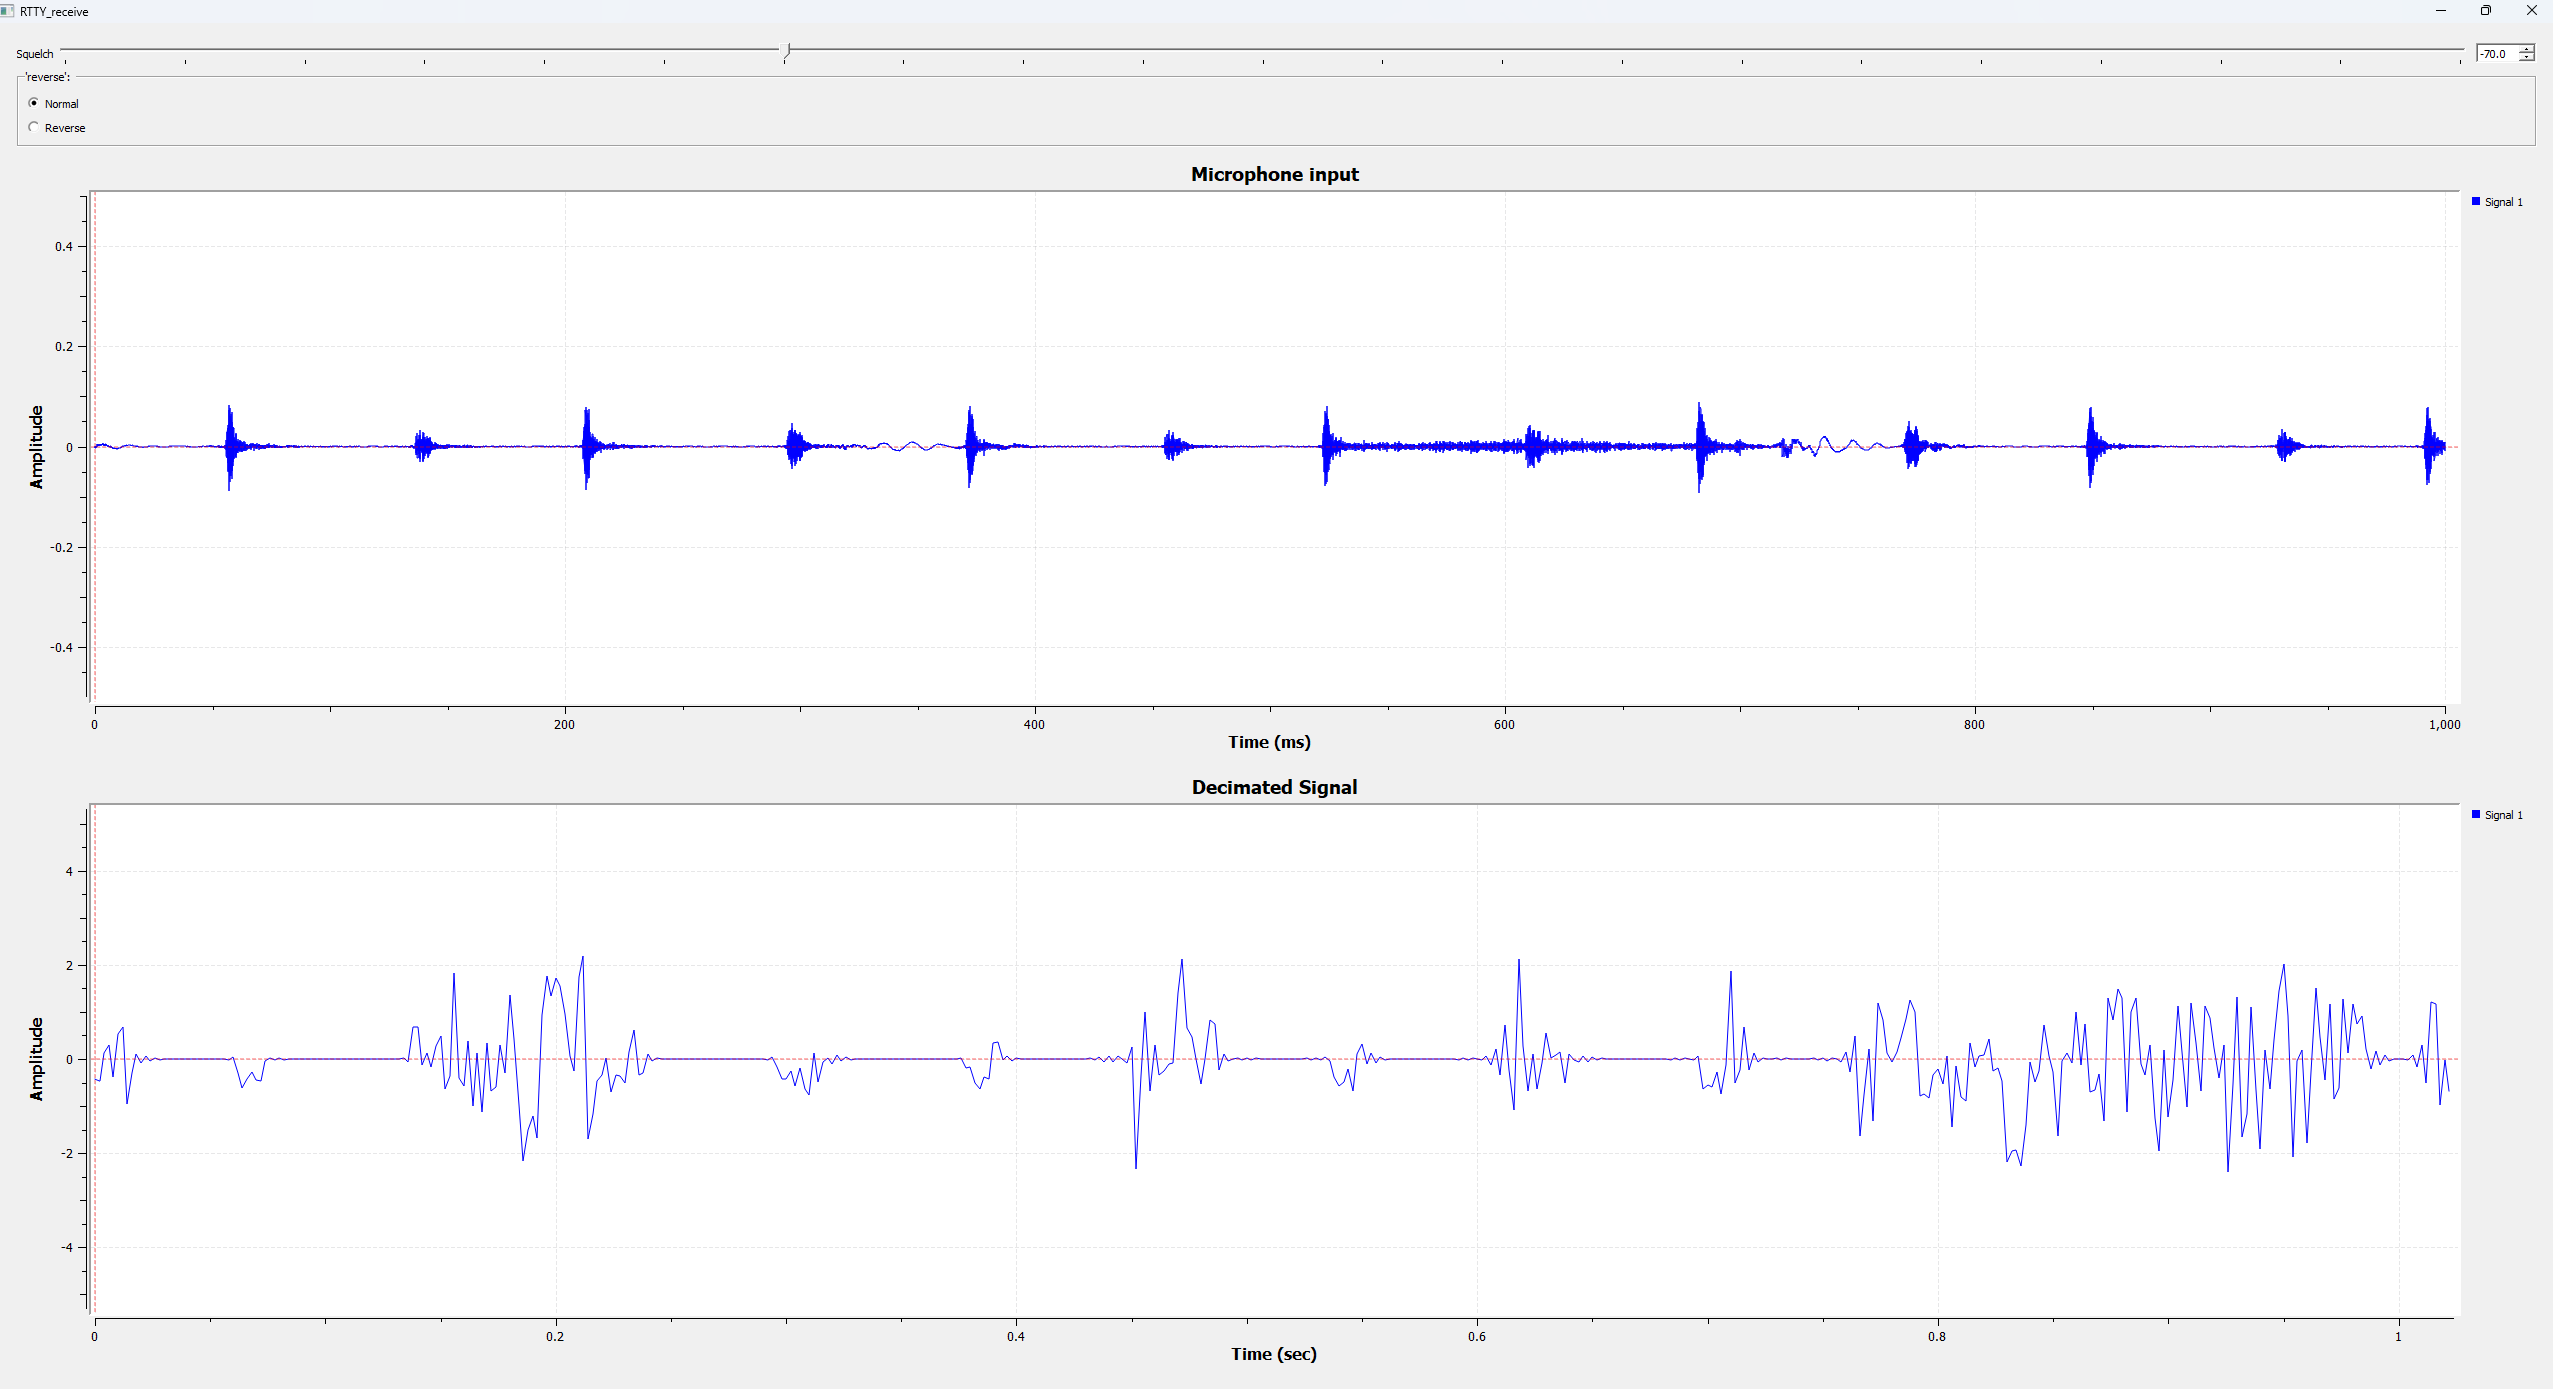
\includegraphics[width=1\textwidth]{images/decim.png}
    \caption{Сигнал до и после децимации}
\end{figure}

\pagebreak

\end{document}
